\chapter{Aufgabe 5}

\begin{figure}
    \centering
    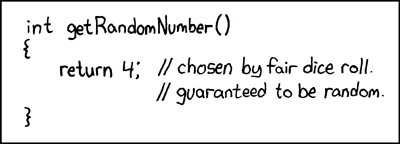
\includegraphics[scale=0.6]{aufgabe 5/img/xkcd221}
    \caption{(Quelle: \url{https://xkcd.com/221/})}
    \label{fig:xkcd221}
\end{figure}


\section{a)}

\textit{Wir betrachten den Pseudozufallsgenerator $x_{i+1} = (a \cdot x_i + b) \ \text{MOD}\ m$ mit Modul
$m = 24$. Für welche Parameter $a,b \in \{1, \ldots, 23\}$ wird die maximale Periodendauer
erreicht?}\\

\noindent
Wir suchen $d$, für das

\begin{equation}\notag
    f^{d+1}(x) = f^i(x), \forall i \geq 0 \qquad{\text{(keine Vorperiode vorhanden)}}
\end{equation}

\noindent
ist.\\

\noindent
\textit{Horster und Schartner} weisen in~\cite[83]{ITS3} auf 3 Bedingungen hin, unter deren EInhaltung eine maximale Periodenlänge $d=m$ garantiert werden kann.
Diese wenden wir im Folgenden an, wobei wir zunächst die Primfaktoren von $m = 24$ bestimmen, die sich trivialerweise zu $\{2, 3\}$ ergeben ($2^3 \cdot 3 = 24$)

\begin{enumerate}
    \itemsep0.5em
    \item Die Werte $m$ und $b$ müssen den größten gemeinsamen Teiler 1 besitzen.
    \item Alle Primfaktoren von $m$ müssen auch $a-1$ teilen.
    \item Ist $m$ durch 4 teilbar, so muss dies auch für $a-1$ gelten.
\end{enumerate}

\noindent
Wir ermitteln zunächst $a$ unter Berücksichtigung von Bedingung 2. und 3.
Da $4|24$ erfüllt ist, suchen wir ein $a-1$, für das $4|a-1$ (Bedingung 3.) sowie  $2|a-1$ und $3|a-1$ gilt (Bedingung 2.).\\
Wir setzen demnach

\begin{equation}\notag
    a=13
\end{equation}

\noindent
Dies ist gleichzeitig der einzige Wert, den wir unter o.a. Bedingungen wählen können.

\noindent
Wir suchen nun nach einem $b$, für das $gcd(b, 24) = 1$ gilt.
Wir können demnach einen Wert aus $\{1, 5, 7, 11, 13, 17, 19, 21, 23\}$ für $b$ auswählen.

\noindent
Damit folgt insgesamt: Für die Werte $a = 13$ und $b \in \{1, 5, 7, 11, 13, 17, 19, 21, 23\}$ wird die maximale Periodenlänge erreicht.


\section{b)}


\noindent
Wir setzen wie folgt ein

\begin{equation}\notag
$x_{i+1} = (13 \cdot x_i + 7) \ \text{MOD}\ 24$
\end{equation}

\noindent
und erhalten mit $x_0 = 0$:

\begin{equation}\notag
    \begin{alignat}{3}
        x_0 &= 0 \\
        x_1 &= (13 \cdot 0 + 5) \ \text{MOD}\ 24 && = 5 \\
        x_2 &= (13 \cdot 5 + 5) \ \text{MOD}\ 24 && = 22 \\
        x_3 &= (13 \cdot 22 + 5) \ \text{MOD}\ 24 && = 3 \\
        x_4 &= (13 \cdot 3 + 5) \ \text{MOD}\ 24 && = 20 \\
        x_5 &= (13 \cdot 20 + 5) \ \text{MOD}\ 24 && = 1 \\
        x_6 &= (13 \cdot 1 + 5) \ \text{MOD}\ 24 && = 18 \\
        x_7 &= (13 \cdot 18 + 5) \ \text{MOD}\ 24 && = 23 \\
        x_8 &= (13 \cdot 23 + 5) \ \text{MOD}\ 24 && = 16 \\
        x_9 &= (13 \cdot 16 + 5) \ \text{MOD}\ 24 && = 21 \\
        x_{10} &= (13 \cdot 21 + 5) \ \text{MOD}\ 24 && = 14 \\
        x_{11} &= (13 \cdot 14 + 5) \ \text{MOD}\ 24 && = 19 \\
        x_{12} &= (13 \cdot 19 + 5) \ \text{MOD}\ 24 && = 12 \\
        x_{13} &= (13 \cdot 12 + 5) \ \text{MOD}\ 24 && = 17 \\
        x_{14} &= (13 \cdot 17 + 5) \ \text{MOD}\ 24 &&= 10\\
        x_{15} &= (13 \cdot 10 + 5) \ \text{MOD}\ 24 &&= 15\\
        x_{16} &= (13 \cdot 15 + 5) \ \text{MOD}\ 24 &&=  8\\
        x_{17} &= (13 \cdot  8 + 5) \ \text{MOD}\ 24 &&= 13\\
        x_{18} &= (13 \cdot 13 + 5) \ \text{MOD}\ 24 &&=  6\\
        x_{19} &= (13 \cdot  6 + 5) \ \text{MOD}\ 24 &&= 11\\
        x_{20} &= (13 \cdot 11 + 5) \ \text{MOD}\ 24 &&=  4\\
        x_{21} &= (13 \cdot  4 + 5) \ \text{MOD}\ 24 &&=  9\\
        x_{22} &= (13 \cdot  9 + 5) \ \text{MOD}\ 24 &&=  2\\
        x_{23} &= (13 \cdot  2 + 5) \ \text{MOD}\ 24 &&=  7\\
        x_{24} &= (13 \cdot  7 + 5) \ \text{MOD}\ 24 &&=  0
    \end{alignat}
\end{equation}

\noindent
Die Periodenlänge dieser Pseudozufallsfolge beträgt 24.


\section{c)}

\textit{Gegeben sei der Öffentliche Schlüssel eines RSA‐Systems $(e, n) = (3, 2773)$. Bestimmen Sie die ersten 10 Bits,
    die von einem RSA‐basierten Pseudozufallsgenerator
ausgegeben werden, wenn der Startwert $s = 5$ gewählt wird.}\\


\noindent
Wir berechnen wie folgt (vgl.~\cite[88]{ITS3}):

\begin{equation}\notag
\begin{alignat}{3}
    5^3 \ \text{MOD} \ 2773 &= 125 \rightarrow \text{lsb} &&= 1\\
    125^3 \ \text{MOD} \ 2773 &= 933 \rightarrow \text{lsb} &&= 1\\
    933^3 \ \text{MOD} \ 2773 &= 1678 \rightarrow \text{lsb} &&= 0\\
    1678^3 \ \text{MOD}\  2773 &= 2708      \rightarrow \text{lsb} &&= 0\\
    2708^3 \ \text{MOD}\  2773 &= 2675      \rightarrow \text{lsb} &&= 1\\
    2675^3 \ \text{MOD}\  2773 &= 1628      \rightarrow \text{lsb} &&= 0\\
    1628^3 \ \text{MOD}\  2773 &= 1103      \rightarrow \text{lsb} &&= 1\\
    1103^3 \ \text{MOD}\  2773 &= 1248      \rightarrow\text{lsb} &&= 0\\
    1248^3 \ \text{MOD}\  2773 &= 139      \rightarrow \text{lsb} &&= 1\\
    139^3 \ \text{MOD}\  2773 &= 1355   \rightarrow\text{lsb} &&= 1
\end{alignat}
\end{equation}


\noindent
Damit ergeben sich die ersten 10 Bits zu

\begin{equation}\notag
    1100\ 1010\  11
\end{equation}


\section{d)}

\textit{Welche Periodendauer besitzt der Pseudozufallsgenerator [Anm.: Abbildung laut Aufgabenstellung], wenn alle
Register zunächst mit einer 1 belegt werden?}

\noindent
Für die Funktion des  rückgekoppelten Schieberegisters ergibt sich

\begin{equation}\notag
    f(z_5, z_4, z_3, z_2, z_1) = z_5 \oplus (z_4 \oplus (z_2 \oplus z_1))
\end{equation}


\noindent
Damit berechnen sich die Inhalte des Schieberegisters schrittweise wie in Tabelle~\ref{tab:schieberegister} angegeben.
Die Periodendauer beträgt $2^5 - 1 = 31$, und ist damit maximal ($2^5$ ist wegen dem stabilen Zustand $00000$ \textit{nicht} die maximale Periodendauer, siehe hierzu~\cite[\textbf{Lösung zu Aufgabe 6.2}, 111]{ITS3}).

\begin{table}[h!]
    \centering
    \setlength{\tabcolsep}{0.5em}
    \begin{tabular}{|c|c|c|c|c|c|c|}
        \hline
        \textbf{} & \textbf{$z_5$} & \textbf{$z_4$} & \textbf{$z_3$} & \textbf{$z_2$} & \textbf{$z_1$} & \textbf{$z_5 \oplus (z_4 \oplus (z_2 \oplus z_1))$} \\
        \hline
        1 &  1 & 1 & 1 & 1 & 1 & 0 \\
        \hline
        2 &  0 & 1 & 1 & 1 & 1 & 1 \\
        \hline
        3 &  1 & 0 & 1 & 1 & 1 & 1 \\
        \hline
        4 &  1 & 1 & 0 & 1 & 1 & 0 \\
        \hline
        5 &  0 & 1 & 1 & 0 & 1 & 0 \\
        \hline
        6 &  0 & 0 & 1 & 1 & 0 & 1 \\
        \hline
        7 &  1 & 0 & 0 & 1 & 1 & 1 \\
        \hline
        8 &  1 & 1 & 0 & 0 & 1 & 1 \\
        \hline
        9 &  1 & 1 & 1 & 0 & 0 & 0 \\
        \hline
        10 &  0 & 1 & 1 & 1 & 0 & 0 \\
        \hline
        11 &  0 & 0 & 1 & 1 & 1 & 0 \\
        \hline
        12 &  0 & 0 & 0 & 1 & 1 & 0 \\
        \hline
        13 &  0 & 0 & 0 & 0 & 1 & 1 \\
        \hline
        14 &  1 & 0 & 0 & 0 & 0 & 1 \\
        \hline
        15 &  1 & 1 & 0 & 0 & 0 & 0\\
        \hline
        16 &  0 & 1 & 1 & 0 & 0 & 1 \\
        \hline
        17 &  1 & 0 & 1 & 1 & 0 & 0 \\
        \hline
        18 &  0 & 1 & 0 & 1 & 1 & 1 \\
        \hline
        19 &  1 & 0 & 1 & 0 & 1 & 0 \\
        \hline
        20 &  0 & 1 & 0 & 1 & 0 & 0 \\
        \hline
        21 &  0 & 0 & 1 & 0 & 1 & 1 \\
        \hline
        22 &  1 & 0 & 0 & 1 & 0 & 0  \\
        \hline
        23 &  0 & 1 & 0 & 0 & 1 & 0  \\
        \hline
        24 &  0 &  0 & 1 & 0 & 0 & 0  \\
        \hline
        25 &  0 &  0 &  0 & 1 & 0 & 1  \\
        \hline
        26 &  1 & 0 &  0 &  0 & 1 & 0 \\
        \hline
        27 &  0 & 1 & 0 &  0 &  0 & 1 \\
        \hline
        28 &  1 & 0 & 1 & 0 &  0 &  1  \\
        \hline
        29 &  1 &  1 & 0 & 1 & 0 &  1  \\
        \hline
        30 &  1 & 1 &  1 & 0 & 1 & 1 \\
        \hline
        31 &  1 & 1 & 1 &  1 & 0 & 1  \\
        \hline
        32 &  1 & 1 & 1 & 1 &  1 & 0 \\
        \hline
    \end{tabular}
    \caption{(Funktions-)Werte des Schieberegister aus Aufgabe 5 d) (Quelle: eigene)}
    \label{tab:schieberegister}
\end{table}